\section{Weierstrass-Enneper Representations}

Having laid the foundations of the complex analysis required, we can now proceed and show how to use these new tools to explore minimal surfaces. We will first introduce isothermal parameters on a minimal surface, show the connection between minimal surfaces and harmonic functions and finally come to Weierstrass-Enneper Representations which is the powerful tool that will allow us to create minimal surfaces with ease.

\subsection{Isothermal Parameters}
\begin{definition}
A parametrisation $\mathbf x(u,v)$ is isothermal if the coefficients of the first fundamental form are of the form:
\begin{displaymath}
E = G, \ \ F = 0
\label{defisothermal}
\end{displaymath}

Geometrically this means angles in the plane look exactly the same as angles on a surface with a isothermal parametrisation. We call this angle preserving.
\end{definition}

\begin{theorem}
Isothermal coordinates exist on all surfaces.
\label{isothermal}
\end{theorem}

We will only prove the case for minimal surfaces as this is all we require. 
\begin{proof}
\cite{OSS}
Fix a point $m \in M$. Choose a coordinate system for $\mathbb R^3$ so that $m$ is the origin, the tangent plane to $M$, $T_mM$, is the $xy$-plane, and near $m$, $M$ is the graph of a function $z=f(x,y)$. Furthermore, the quotient and chain rules give

\begin{displaymath}
\left(\frac{1+f_x^2}{w}\right)_y-\left(\frac{f_xf_y}{w}\right)x = -\frac{f_y}{w}\left[f_{xx}(1+f^2_y)-2f_xf_yf_{xy}+f_{yy}(1+f^2_x)\right]
\end{displaymath}

\begin{displaymath}
\left(\frac{1+f_y^2}{w}\right)_x-\left(\frac{f_xf_y}{w}\right)y = -\frac{f_x}{w}\left[f_{xx}(1+f^2_y)-2f_xf_yf_{xy}+f_{yy}(1+f^2_x)\right]
\end{displaymath}

where $w=\sqrt{1+f_x^2+f_y^2}$. Let $p=f_x$, $q=f_y$ with $w^2 = 1 + p^2 + q^2$. Because $M$ is minimal, $f$ satisfies the \emph{Minimal Surface Equation}

\begin{displaymath}
f_{xx}(1+f_y^2)-2f_xf_yf_{xy}+f_{yy}(1+f_x^2)=0,
\end{displaymath}

so we have $\left(\frac{1+p^2}{w}\right)_y - \left(\frac{pq}{w}\right)_x = 0$ and $\left(\frac{1+q^2}{w}\right)_x - \left(\frac{pq}{w}\right)_y = 0$. Define two vector fields in the $xy$-plane by
\begin{displaymath}
V=\left(\frac{1+p^2}{w},\frac{pq}{w}\right) \mbox{\ \ \ \ and \ \ \ \ } W=\left(\frac{pq}{w},\frac{1+q^2}{w}\right)
\end{displaymath}
and apply Green's theorem to any closed curve C contained in a simply connected region $\it{R}$ to obtain

\begin{displaymath}
\int_C V\cdot dr = \int \int_{\it{R}}\left(\frac{pq}{w}\right)_x-\left(\frac{1+p^2}{w}\right)_y dxdy=0,
\end{displaymath}

\begin{displaymath}
\int_C W\cdot dr = \int \int_{\it{R}}\left(\frac{1+q^2}{w}\right)_x - \left(\frac{pq}{w}\right)_y dxdy=0,
\end{displaymath}

where $dr = (dx,dy)$. Since the line integrals are zero for all closed curves in $\it R$, $V$ and $W$ must have potential functions (see \cite{MT}). That is, there exist $\mu$ and $\rho$  with $\mbox{grad }(\mu)= V$ and $\mbox{grad }(\rho) = W$. Considered coordinatewise, these equations imply $\mu_x = \frac{1+p^2}{w}$, $\mu_y=\frac{pq}{w}$ and $\rho_x = \frac{pq}{w}$, $\rho_y = \frac{1+q^2}{w}$. Define a mapping $T:\it R \rightarrow \mathbb R^2$ by

\begin{displaymath}
T(x,y) = (x+\mu(x,y),y+\rho(x,y)).
\end{displaymath}

The Jacobian matrix of this mapping is then
\begin{displaymath}
J(T)= \left[ \begin{array}{cc}
1+\mu_x & \rho_y \\
\rho_x & 1+\rho_y
\end{array} \right] = \left[ \begin{array}{cc}
1+\frac{1+p^2}{w} & \frac{pq}{w} \\
\frac{pq}{w} & 1+ \frac{1+q^2}{w}
\end{array} \right],
\end{displaymath}

and we calculate the determinant to be $det(J(T)) = \frac{(1+w)^2}{w} > 0$. The Inverse Function Theorem then says that, near $m=(0,0)$, there is a smooth inverse function $T^{-1}(u,v)=(x,y)$ with

\begin{eqnarray}
\nonumber
J(T^{-1})&=&J(T)^{-1} \\
\nonumber
&=&\frac{1}{\mbox{det }J(T)}\left[ \begin{array}{cc}
1+\frac{1+p^2}{w} & \frac{pq}{w} \\
\frac{pq}{w} & 1+ \frac{1+q^2}{w}
\end{array} \right] \\
\nonumber
&=&\frac{1}{(1+w)^2}\left[ \begin{array}{cc}
w+1+q^2 & pq \\
-pq & 1+ w+1+p^2
\end{array} \right]
\end{eqnarray}

Of course, for $(x,y) = T^{-1}(u,v)$, the last matrix is just
\begin{displaymath}
\left[ \begin{array}{cc}
x_u & x_v \\
y_u & y_v
\end{array} \right]
\end{displaymath}
by the definition of the Jacobian. We will put these calculations to use in showing that the parametrisation (in the $u,v$ coordinates described above) $\mathbf x(u,v) \stackrel{def}{=}(x(u,v),\ y(u,v),\ f(x(u,v),y(u,v)))$ is isothermal.

First calculate

\begin{eqnarray}
\nonumber
\mathbf x_u &=& \left(\frac{w+1+q^2}{(1+w)^2},\frac{-pq}{(1+w)^2},p\left(\frac{w+1+q^2}{(1+w)^2}\right)+q\left(\frac{-pq}{(1+w)^2}\right)\right) \\
\nonumber
\mathbf x_u &=& \left(\frac{-pq}{(1+w)^2},\frac{w+1+p^2}{(1+w)^2},p\left(\frac{(-pq)(w+1+q^2)}{(1+w)^2}\right)+q\left(\frac{w+1+p^2}{(1+w)^2}\right)\right)
\end{eqnarray}

Now all that remains is to calculate the coefficients of the first fundamental form:

\begin{eqnarray}
\nonumber
E &=& \mathbf x_u \cdot \mathbf x_u \\
\nonumber
&=& \frac{1}{(1+w)^4}[(w+1+q^2)^2 + p^2q^2 +p^2(w+1+q^2)^2 \\
\nonumber
&\ & \ \ \ \ -2p^2q^2(w+1+q^2)+p^2q^4]\\
\nonumber
&=& \frac{1}{(1+w)^4}[(1+w)^2(1+q^2+p^2)] \\
\nonumber
&=& \frac{w^2}{(1+w)^2} \\
\nonumber
G &=& \mathbf x_v \cdot \mathbf x_v \\
\nonumber
&=&\frac{1}{(1+w)^4}[p^2q^2+(w+1+p^2)^2+ p^4q^2 \\
\nonumber
&\ & \ \ \ \ -2q(w+1+p^2)p^2q+q(w+1+p^2)^2] \\
\nonumber
&=&\frac{1}{(1+w)^4}[(1+w)^2(1+q^2+p^2)] \\
\nonumber
&=&\frac{w^2}{(1+w)^2} \\
\nonumber
&=& E
\end{eqnarray}
\begin{eqnarray}
\nonumber
F &=& \mathbf x_u \cdot \mathbf x_v \\
\nonumber
&=&\frac{1}{(1+w)^4}[-(w+1+q^2)pq - pq(w+1+p^2) \\
\nonumber
&\ & \ \ \ \ + (p(w+1+q^2)-q^2p)(-p^2q+q(w+1+p^2))] \\
\nonumber
&=&\frac{1}{(1+w)^4}[-\cancel{pqw}-\cancel{pq}-pq^3-\cancel{pqw}-pq-p^3q+pw^2q+\cancel{2pqw}+\cancel{pq} \\
\nonumber
&=&-pq^3-pq-p^3q+pw^2q \\
\nonumber
&=&-pq^3-pq-p^3q+pq(1+p^2+q^2) \\
\nonumber
&=& 0
\end{eqnarray}   
Hence, the parametrisation $\mathbf x(u,v)$ is isothermal.
\end{proof}

\begin{cor}
If M is a surface with isothermal parametrisation $\mathbf x(u,v)$ the formula for mean curvature reduces to $H=\frac{L+N}{2E}$. Hence, for M to be a minimal surface, $L = -N$
\end{cor}

\subsection{Gauss Equations}
To continue to link Minimal Surface theory to complex analysis we need to set up some identities known as the Gauss Equations (or the Acceleration Formulae in \cite{OPR}). These are formulas that express $\mathbf x_{uu}$, $\mathbf x_{uv}$, $\mathbf x_{vv}$ in an othonormal basis with \emph{Christoffel Symbols} of the 2nd kind as the coefficients, eg they are calculated from the coefficients of the first fundamental form. This follows directly from Gauss's \emph{Theorema Egregium}.

\begin{prop}[Gauss Equations]
\cite{EDG}
Given a surface $\mathbf x(u,v)$, then $\{\mathbf x_u, \mathbf x_v\}$ is an orthonormal basis for the tangent plane and $\mathbf N$ is a unit normal to the tangent plane so clearly $\{\mathbf x_u, \mathbf x_v, \mathbf N\}$ is a basis for $\mathbb{R}^3$. We can then express the second derivatives on the surface as:

\begin{align}
\nonumber
&\mathbf x_{uu}& &=& \Gamma^u_{uu} &\mathbf x_{u}& &+& \Gamma^v_{uu} &\mathbf x_{v}& &+& L &\mathbf N& \\
\nonumber
&\mathbf x_{uv}& &=& \Gamma^u_{uv} &\mathbf x_{u}& &+& \Gamma^v_{uv} &\mathbf x_{v}& &+& M &\mathbf N& \\
\nonumber
&\mathbf x_{vv}& &=& \Gamma^u_{vv} &\mathbf x_{u}& &+& \Gamma^v_{vv} &\mathbf x_{v}& &+& N &\mathbf N&
\end{align}
\end{prop}

\begin{proof}
These coefficients are calculated by manipulating the chain rule on some basic identities.

\begin{eqnarray}
\nonumber
\mathbf x_u \cdot \mathbf x_v &=& 0 \\
\Leftrightarrow \mathbf x_{uu} \cdot \mathbf x_v &=& - \mathbf x_u \cdot \mathbf x_{uv} 
\label{x_uux_v} \\
\Leftrightarrow \mathbf x_{vv} \cdot \mathbf x_{u} &=& -\mathbf x_v \cdot \mathbf x_{uv}
\label{x_vvx_u}
\end{eqnarray}

\begin{eqnarray}
\nonumber
E &=& \mathbf x_u \cdot \mathbf x_u \\
\Leftrightarrow E_u &=& \mathbf x_{uu} \cdot \mathbf x_u + \mathbf x_u \cdot \mathbf x_{uu} = 2 \mathbf x_{uu} \cdot \mathbf x_u
\label{E_u} \\
\Leftrightarrow E_v &=& \mathbf x_{u} \cdot \mathbf x_{uv} + \mathbf x_u \cdot \mathbf x_{uv} = 2 \mathbf x_{u} \cdot \mathbf x_{uv} \stackrel{\ref{x_uux_v}}{=} -2 \mathbf x_{uu} \cdot \mathbf x_v
\label{E_v} \\
\nonumber
&\ & \\
\nonumber
G &=& \mathbf x_v \cdot \mathbf x_v \\
\Leftrightarrow G_u &=& 2 \mathbf x_{uv} \cdot \mathbf x_v \stackrel{\ref{x_vvx_u}}{=} - 2 \mathbf x_{vv} \cdot \mathbf x_{u}
\label{G_u} \\
\Leftrightarrow G_v &=& -2 \mathbf x_{vv} \cdot \mathbf x_v
\label{G_v}
\end{eqnarray}

Using this set of equations we can then work through and calculate each coefficient:

\begin{eqnarray}
\nonumber
\mathbf x_{uu} \cdot \mathbf x_u &=& \Gamma^u_{uu} \mathbf x_u \cdot \mathbf x_u \ \ \ \mbox{(Since $\mathbf x_u \cdot \mathbf x_v$ and $\mathbf N \cdot \mathbf x_u$ equal $0$)}
\\
\nonumber
\Leftrightarrow \Gamma^u_{uu} &\stackrel{\ref{E_u}}{=}& \frac{E_u}{2E}
\\
\nonumber
&\ & \\
\nonumber
\mathbf x_{uu} \cdot \mathbf x_v &=& \Gamma^v_{uu} \mathbf x_v \cdot \mathbf x_v 
\\
\nonumber
\Leftrightarrow \Gamma^v_{uu} &\stackrel{\ref{E_v}}{=}& \frac{E_v}{2G}
\\
\nonumber
&\ & \\
\nonumber
\mathbf x_{uu} \cdot \mathbf N &=& L \mathbf N \cdot \mathbf N
\\
\nonumber
\Leftrightarrow L &=& \mathbf x_{uu} \cdot \mathbf N  \ \ \mbox{Since $\mathbf N \cdot \mathbf N = 1$}
\end{eqnarray}

Following the same method for the remaining coefficients results in:

\begin{align}
&\mathbf x_{uu}& &=& \frac{E_u}{2E} &\mathbf x_{u}& &-& \frac{E_v}{2G} &\mathbf x_{v}& &+& L &\mathbf N& \label {x_uu} \\
&\mathbf x_{uv}& &=& \frac{E_v}{2E} &\mathbf x_{u}& &+& \frac{G_u}{2G} &\mathbf x_{v}& &+& M &\mathbf N& \label{x_uv}\\
&\mathbf x_{vv}& &=& -\frac{G_u}{2E} &\mathbf x_{u}& &+& \frac{G_v}{2G} &\mathbf x_{v}& &+& N &\mathbf N& \label{x_vv}
\end{align}
\end{proof}

\subsection{The Relationship between Minimal Surfaces and \\ Harmonic Functions}
\begin{theorem}
If the parametrisation $\mathbf x$ is isothermal then 
\begin{displaymath}
\mathbf \Delta \mathbf x \stackrel{def}{=} \mathbf x_{uu} + \mathbf x_{vv} = (2EH)\mathbf N
\end{displaymath}
\end{theorem}

\begin{proof} 
This follows simply by subbing in from the Gauss Equations.
\begin{eqnarray}
\nonumber
\mathbf x_{uu} + \mathbf x_{vv} &=& \stackrel{\ref{x_uu}}{(\frac{E_u}{2E} \mathbf x_{u} - \frac{E_v}{2G} \mathbf x_{v} + L \mathbf N)} + \stackrel{\ref{x_vv}}{(-\frac{G_u}{2E} \mathbf x_{u} + \frac{G_v}{2G} \mathbf x_{v} + N \mathbf N)} 
\\
\nonumber
&=& (L+N)\mathbf N 
\\
\nonumber
&=& 2 E \left(\frac{L+N}{2E} \right)\mathbf N 
\\
\nonumber
&=& (2EH)\mathbf N
\end{eqnarray}
\end{proof}

\begin{cor}
A surface $S$ with an isothermal parametrisation is minimal if and only if its coordinate functions are harmonic.
\label{harmonic}
\end{cor}

\begin{proof}
If S is minimal, $H = 0$ and so clearly $\mathbf x_{uu} + \mathbf x_{vv} = 0$. Conversely if the coordinate function of $S$ are harmonic then $\mathbf x_{uu} + \mathbf x_{vv} = 0$ and so $(2EH) \mathbf N = 0$. $\mathbf N$ is the unit normal and $E \neq 0$ so $H=0$ and $S$ is minimal.
\end{proof}

From complex analysis we know that given a harmonic function $X$ we can immediately produce a conjugate harmonic function $Y$, which defines a complex analytic function $Z = X + i Y$ (See example \ref{Enneper}). Taking the harmonic coordinate functions for our minimal surface $\mathbf x$ we can produce a harmonic conjugate for each $\mathbf x^j$ giving us a new minimal surface $\mathbf y$. We therefore can define a set of complex analytic function $\mathbf Z^j = \mathbf x^j + i \mathbf y^j$. Multiplying by $e^{i\theta} (= \cos(\theta)+i\sin(\theta))$ rotates the real part of $\mathbf Z$ into the imaginary part and vice versa. Taking the real or imaginary part of $\mathbf Z$ as we perform this rotation produces a one parameter family of surfaces that maps $\mathbf x$ into $\mathbf y$.

\begin{theorem}
The one parameter family of surfaces that exists between any minimal surface and its conjugate minimal surface are all minimal.
\end{theorem}

\begin{proof}
We will use the fact that a surface is minimal (with isothermal coordinates) if and only if its coordinate functions are harmonic.
Let $\mathbf x(u,v)$ be a minimal surface with $\mathbf y(u,v)$ its harmonic conjugate surface. By definition of a minimal surface:

\begin{displaymath}
\frac{\partial^2 \mathbf x^j}{\partial u^2}+\frac{\partial^2 \mathbf x^j}{\partial v^2}=0 \ \
\frac{\partial^2 \mathbf y^j}{\partial u^2}+\frac{\partial^2 \mathbf y^j}{\partial v^2}=0
\end{displaymath}

Starting from
\begin{eqnarray}
\nonumber
\mathbf Z(u,v) &=& e^{i\theta}(\mathbf x + i \mathbf y)
\\
\nonumber
&=& (\cos \theta + i \sin \theta)(\mathbf x + i \mathbf y)
\\
&=& (\mathbf x \cos \theta - \mathbf y \sin \theta) + i(\mathbf x \cos \theta + \mathbf y \sin \theta)
\label{Z} 
\end{eqnarray} 

So we want the real and imaginary parts of \ref{Z} to be harmonic which implies that they define minimal surfaces by Corollary \ref{harmonic}.

\begin{eqnarray}
\nonumber
\frac{\partial^2 \Re(\mathbf Z)}{\partial u^2} + \frac{\partial^2 \Re(\mathbf Z)}{\partial v^2} &=& \left ( \frac{\partial^2 \mathbf x}{\partial^2 u} \cos \theta - \frac{\partial^2 \mathbf y}{\partial^2 u} \sin \theta \right ) + \left ( \frac{\partial^2 \mathbf x}{\partial^2 v} \cos \theta - \frac{\partial^2 \mathbf y}{\partial^2 v} \sin \theta \right )
\\
\nonumber
&=& \cos\theta \left (\frac{\partial^2 \mathbf x}{\partial^2 u} + \frac{\partial^2 \mathbf x}{\partial^2 v} \right ) - \sin\theta \left (\frac{\partial^2 \mathbf y}{\partial^2 u} + \frac{\partial^2 \mathbf y}{\partial^2 v} \right )
\\
\nonumber
&=& 0 \mbox{\ \ \ Since $\mathbf x$ and $\mathbf y$ and both harmonic.}
\end{eqnarray}

\begin{eqnarray}
\nonumber
\frac{\partial^2 \Im(\mathbf Z)}{\partial u^2} + \frac{\partial^2 \Im(\mathbf Z)}{\partial v^2} &=& \left ( \frac{\partial^2 \mathbf x}{\partial^2 u} \sin \theta + \frac{\partial^2 \mathbf y}{\partial^2 u} \cos \theta \right ) + \left ( \frac{\partial^2 \mathbf x}{\partial^2 v} \sin \theta + \frac{\partial^2 \mathbf y}{\partial^2 v} \cos \theta \right )
\\
\nonumber
&=& \sin\theta \left (\frac{\partial^2 \mathbf x}{\partial^2 u} + \frac{\partial^2 \mathbf x}{\partial^2 v} \right ) + \cos\theta \left (\frac{\partial^2 \mathbf y}{\partial^2 u} + \frac{\partial^2 \mathbf y}{\partial^2 v} \right )
\\
\nonumber
&=& 0 \mbox{\ \ \ Since $\mathbf x$ and $\mathbf y$ and both harmonic.}
\end{eqnarray}
\end{proof}

\begin{example}[Ennepers Surface]
\label{Enneper}
Ennepers Surface is parametrized by 
\begin{displaymath}
\mathbf x(u,v) = (u-\frac{1}{3}u^3 + uv^2)\mathbf e_x + (-v-u^2v+\frac{1}{3}v^3)\mathbf e_y + (u^2-v^2)\mathbf e_z
\end{displaymath}

It is easy to check that $E=G$ and $F=0$ therefore the parametrisation is isothermal.

I will demonstrate the method of checking that $\mathbf x$ is harmonic and calculating it's harmonic conjugate with the z coordinate function.

\begin{eqnarray}
\nonumber
\frac{\partial \mathbf x^3}{\partial u}=\frac{\partial \mathbf y^3}{\partial v} \Leftrightarrow \frac{\partial \mathbf y^3}{\partial v} &=& 2u \\
\nonumber
\therefore \mathbf y^3 &=& 2uv + f(u) \\
\nonumber
\frac{\partial \mathbf x^3}{\partial v}=-\frac{\partial \mathbf y^3}{\partial u} \Leftrightarrow 2v + f'(u) &=& 2v \\
\nonumber
f'(u) &=& 0 \\
\nonumber
\Leftrightarrow f(u) &=& k \\
\nonumber
\therefore \mathbf y^3 &=& 2uv + k
\end{eqnarray}

Carrying this procedure out on each coordinate function generates a conjugate harmonic surface (note we ignore additive constants):
\begin{displaymath}
\mathbf y(u,v) = (v-vu^2+\frac{1}{3}v^3)\mathbf e_x + (u+\frac{1}{3}u^3-uv^2)\mathbf e_y + 2uv \mathbf e_z
\end{displaymath}

We can now define a function $\mathbf Z = \mathbf x + i \mathbf y$. Multiplying this by $\cos\theta + i \sin\theta$ and taking the real part (or equally the imaginary part) gives us a one parameter family of surfaces.

At the turning points of $\sin \theta$  and $\cos \theta$ $\Re (\mathbf Z)$ becomes
\begin{align}
\nonumber
&\theta = 0& &\Leftrightarrow& &\mathbf x& \\
\nonumber
&\theta = \frac{\pi}{2}& &\Leftrightarrow& -&\mathbf y&  \\
\nonumber
&\theta = \pi& &\Leftrightarrow& -&\mathbf x& \\
\nonumber
&\theta = \frac{2\pi}{2}& &\Leftrightarrow& &\mathbf y& \\
\nonumber
&\theta = 2\pi& &\Leftrightarrow& &\mathbf x&
\end{align}

Some of this family is shown in Figure \ref{fig:enneper}.

\begin{figure}[htbp]
	\centering
       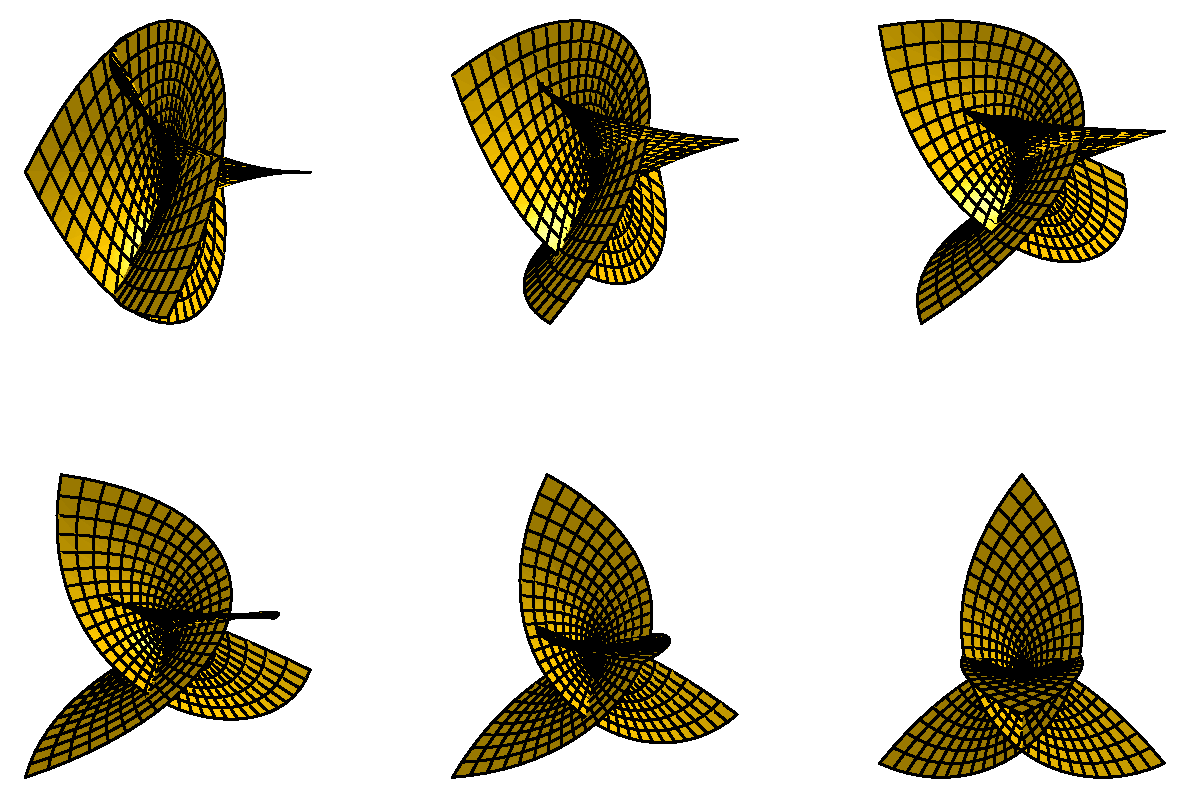
\includegraphics[width=12cm]{Images/EnneperFamily.eps}
   \caption{The Enneper Family of Minimal Surfaces}
   \label{fig:enneper}
\end{figure}

\end{example} 

\subsection{The Weierstrass-Enneper Representation}
\label{WERep}
We know all surfaces can be isothermally parametized (\ref{defisothermal}) and if an isothermally parametrised surface is minimal then its coordinate functions are harmonic (\ref{harmonic}).

Let $\mathbf x(u,v)$ be a minimal surface with an isothermal parametrisation (Section \ref{isothermal})

Then let $\mathbf y$ be the harmonic conjugate of $\mathbf x$.

Using the complex variable $z = u + iv$ we can write
\begin{displaymath}
\mathbf f(z) = \mathbf x + i \mathbf y \mbox{\ \ is holomorphic}
\end{displaymath}

Now define $\mathbf \Phi$ as

\begin{displaymath}
\mathbf \Phi = \frac{\partial \mathbf f}{\partial z} = \frac{1}{2}(\mathbf x_u + i \mathbf y_u) \stackrel{\ref{CR}}{=} \frac{1}{2}(\mathbf x_u - i \mathbf x_v) 
\label{Phi}
\end{displaymath}

\begin{theorem}
If $\mathbf \Phi: U \rightarrow \mathbb R^3$ is an isothermally parametrised minimal surface, the vector-valued holomorphic function $\mathbf \Phi=(\Phi_1, \Phi_2, \Phi_3)$ defined above satisfies the following conditions:
\begin{enumerate}
	\item $\Phi_1^2+\Phi_2^2+\Phi_3^2 = 0$ 
	\item $\mathbf \Phi$ is nowhere zero.
\end{enumerate}
\end{theorem}

\begin{proof}
\begin{eqnarray}
\nonumber
\sum_{k=1}^3 \Phi_k^2 &=& \sum_{k=1}^3 \frac{1}{4}\left(x_u^k - i x_v^k \right) \\
\nonumber
&=& \frac{1}{4}(\mathbf x_u \cdot \mathbf x_u - \mathbf x_v \cdot \mathbf x_v - 2i \mathbf x_u \cdot \mathbf x_v) \\
\nonumber
&=& \frac{1}{4}(E - G - 2i F) \\
\nonumber
&=& 0 \mbox{\ \ by definition of isothermal paramatization (\ref{defisothermal})}
\end{eqnarray}
Finally $\mathbf \Phi = \vec 0$ iff $\mathbf x_u = \mathbf x_v = 0$ which is impossible since $\mathbf x$ is regular.
\end{proof}

Now if we define

\begin{displaymath}
g(z) = \frac{\Phi_3}{\Phi_1-i\Phi_2} \mbox{\ and \ } f(z) = \Phi_1-i\Phi_2
\end{displaymath} 

Manipulating these gives:

\begin{eqnarray}
\nonumber
\Phi_1 &=& \frac{1}{2}(1-g^2)f \\
\nonumber
\Phi_2 &=& \frac{i}{2}(1+g^2)f \\
\nonumber
\Phi_3 &=& fg\\
\end{eqnarray}

Note these satisfy $\Phi_1^2+\Phi_2^2+\Phi_3^2 = 0$.
 
We can take a path independent contour integral for each $\Phi_i$ with respect to z. The real part of which will be our isothermally parametrised minimal surface $\mathbf x(u,v)$ and the imaginary part will be the harmonic conjugate minimal surface, $\mathbf y(u,v)$.\\
Conditions on g:
\begin{enumerate}
	\item Meromorphic
\end{enumerate}
Conditions on f:
\begin{enumerate}
	\item Holomorphic
	\item If g has a pole of order $m \geq 1$ at $z_0$ then f has a zero of order $n \geq 2m$ at $z_0$.
\end{enumerate}

\begin{example}
To demonstrate the ease with which we can now produce minimal surfaces we will take,
\begin{displaymath}
f(z) = z \ \ \ \ g(z) = z
\end{displaymath}

So 

\begin{eqnarray}
\nonumber
\Phi_1 &=& \frac{1}{2}(1-z^2)z \\
\nonumber
\Phi_2 &=& \frac{i}{2}(1+z^2)z \\
\nonumber
\Phi_3 &=& z^2
\end{eqnarray}

Then
\begin{eqnarray}
\nonumber
x^1(z,\bar{z}) &=& \Re \int \Phi_1 dz \\
\nonumber
&=& \Re \left(\frac{1}{8}(2z^2-z^4)\right) \mbox{\ \ \ \ Now sub in for } z=u+iv \\
\nonumber
&=& -\frac{1}{4}u^4+\frac{3}{2}u^2v^2-\frac{1}{4}v^4+\frac{1}{2}u^2-\frac{1}{2}v^2
\end{eqnarray}

\begin{eqnarray}								
\nonumber
x^2(z,\bar{z}) &=& \Re \int \Phi_2 dz \\
\nonumber
&=& \Re \left(\frac{i}{8}(2z^2+z^4)\right) \mbox{\ \ \ \ Now sub in for } z=u+iv \\
\nonumber
&=& u^3v+uv^3-uv
\end{eqnarray}

\begin{eqnarray}								
\nonumber
x^3(z,\bar{z}) &=& \Re \int \Phi_3 dz \\
\nonumber
&=& \Re \left(\frac{z^3}{3}\right) \mbox{\ \ \ \ Now sub in for } z=u+iv \\
\nonumber
&=& \frac{2}{3}u^3-2v^2u
\end{eqnarray} 
\end{example}

So we have a minimal surface $\mathbf x(u,v) = (x^1,x^2,x^3)$ which is shown in Figure \ref{fig:WEExample}.

\begin{figure}[htbp]
	\centering
       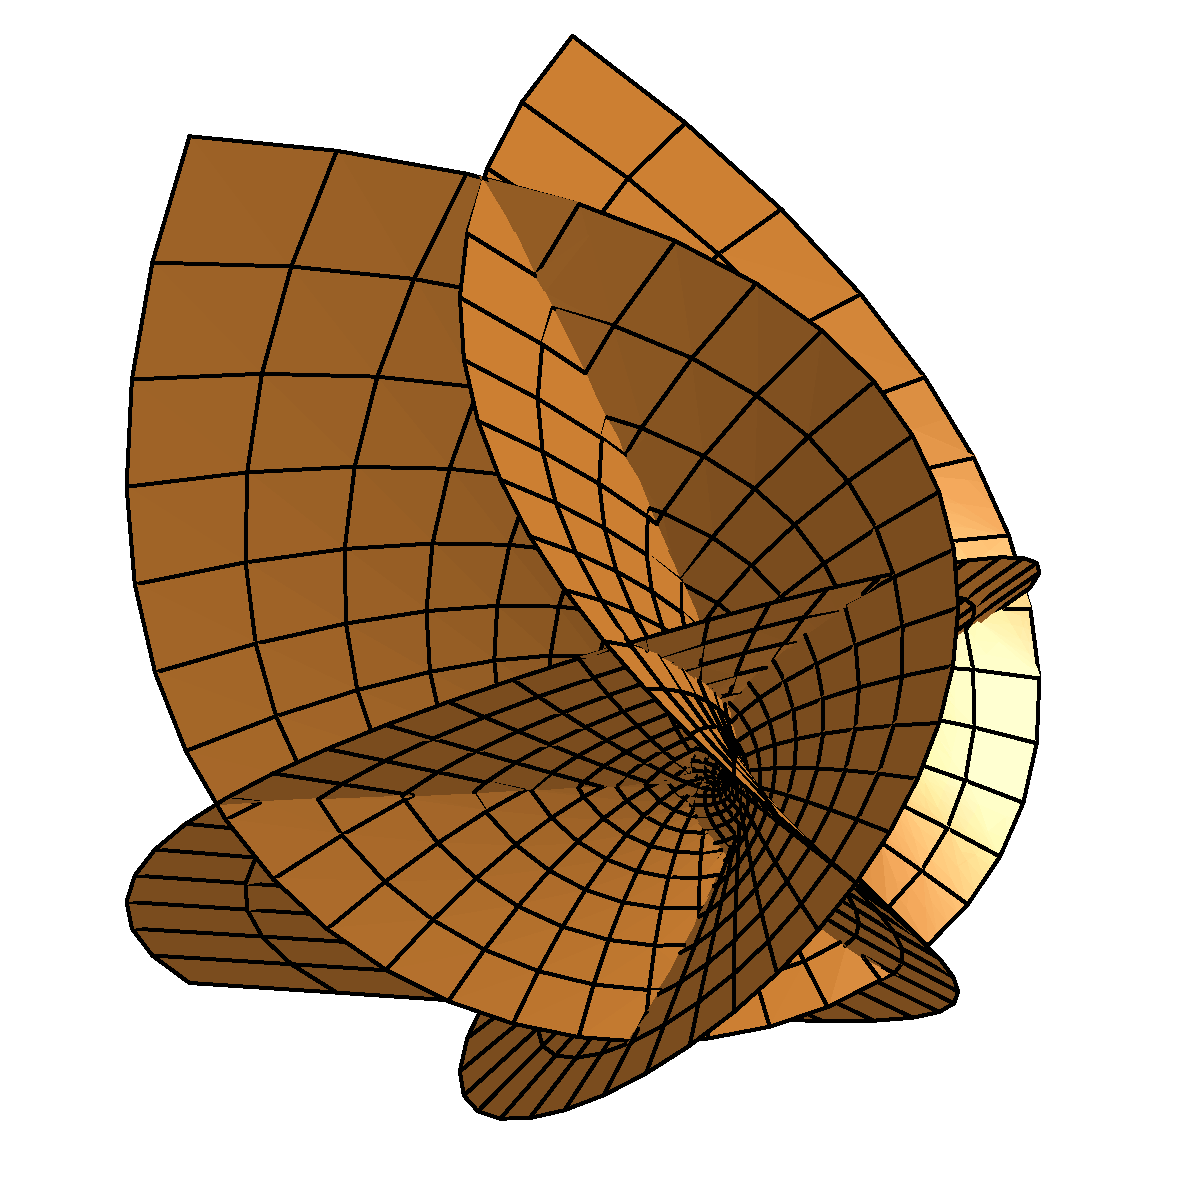
\includegraphics[width=8cm]{Images/WEExample.eps}
   \caption{Minimal Surface Generated by $f(z) = z$ and $g(z) = z$}
   \label{fig:WEExample}
\end{figure}


 

